\item \points{2a} 

Implement both forward-propagation and back-propagation for the above loss function.
Initialize the weights of the network by sampling values from a standard normal
distribution. Initialize the bias/intercept term to 0.
Set the number of hidden units to be 300, and learning rate to be 0.4. Set $B = 1,000$
(mini batch size). This means that we train with 1,000 examples in each iteration.
Therefore, for each epoch, we need 50 iterations to cover the entire training data.
The images are pre-shuffled. So you don't need to randomly sample the data, and can
just create mini-batches sequentially.

Use autograder test case |2aii-6-basic| to train the model with mini-batch gradient descent
as described above. Before running this test case, edit line 186 of |src-mnist/grader.py| to state |skip = False| (model plotting/training is disabled by default to run the auotgrader faster). This will run the training for 30 epochs. At the end of each epoch, it will calculate
the value of loss function averaged over the entire training set.  It will then plot the average loss (y-axis) against the number of epochs (x-axis). In the same image, it will also plot the value of the loss function averaged over the dev set, and against the number of epochs.

This will also plot the accuracy (on y-axis) over the training set,
measured as the fraction of correctly classified examples, versus the number of epochs
(x-axis). In the same image, it will plot the accuracy over the dev set versus number of epochs.

\textbf{Hint:} Be sure to vectorize your code as much as possible! Training can be
very slow otherwise.

\clearpage\newpage

You plots should look similar to the following (You are not required to submit any plots.  These are for your own verification.):

\begin{figure}[H]
    \centering
    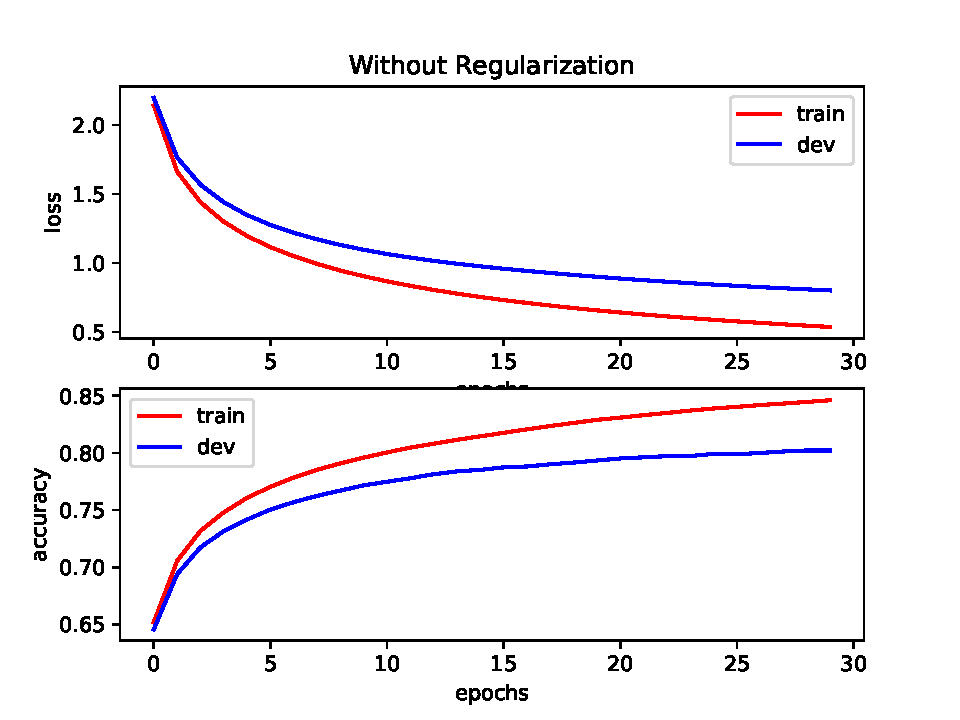
\includegraphics[scale=0.75]{02-mnist/baseline.pdf}
\end{figure}
